\documentclass[12pt]{article}
\usepackage[english]{babel}
\usepackage[utf8x]{inputenc}
\usepackage{amsmath}
\usepackage{graphicx} 		% Used to for importing images
\usepackage{indentfirst}	% Indents 1st paragraph (by default its off)
\usepackage{longtable} 		% Tables than can span over multiple pages
\usepackage{placeins}		% Used to keep images in place(via \FloatBarriers), and let text go infront

% Define Global Variables
\setlength{\parindent}{20pt}
\graphicspath{ {/Diagrams} }

\begin{document}

\begin{titlepage}

% Defines a new command to draw horizontal lines
\newcommand{\Line}{\rule{\linewidth}{0.5mm}} 

% Center everything on the page
\center
 
% textsc - capitalizes every letter
\textsc{\LARGE University of Gothenburg}
% Define gap after text line
\\[3.5cm] 

% Course code and name
\textsc{\Large DIT168}\\[0.3cm]
\textsc{\large Project: Industrial IT and Embedded Systems}\\[0.5cm]

% Use the defined command to draw lines
\Line \\[0.4cm]
{\huge \bfseries Software Architectural Document}\\[0.4cm]
\Line \\[0.5cm]
 
% Large italic text
\Large \textit{Authors:}
\\Erik Laurin
\\Isabelle Törnqvist
\\Joacim Eberlen
\\Justinas Stirbys \\[4cm]

% Original date for the vision
{\large Group 01} \\[0.3cm]
{\large March 30th, 2018}

% Fills the remaining page with whitespace
\vfill

\end{titlepage}

% Creating table of contents
\tableofcontents
\pagebreak

% a SAD start
%%%%%%%%%%%%%%%%%%%%%%%%%%%%%%%%%%
% Add SAD history of changes table
%%%%%%%%%%%%%%%%%%%%%%%%%%%%%%%%%%

\section{Revision History}
The evolution of the Software Architectural Document for project dashFTABs is detailed under this section. Emphasis is put on changes incorporated, via Description column, the date and the author. In situation where all members have contributed to a change the author will be listed as Group 01.
% Define 4 aligned columns; l = left, c = center, r = right, the | = means vertical line    % \hline -> Draw horizontal line
% p{xcm} -> specifies how much space the column should take up, 
% 0.x\linewidth is used to make it p{} command more dynamic
\begin{longtable}{ | p{0.25\linewidth} | p{0.1\linewidth} | p{0.5\linewidth} | p{0.15\linewidth} | }\hline 
    Date & Version & Description & Author \\ \hline
   	27th March, 2018 & 0.1 & Added Functional Requirements & Group 01\\ \hline
   	4th April, 2018 & 0.2 & Added Introduction & Justinas\\ \hline
   	5th April, 2018 & 0.3 & Added Use Case View & Justinas\\ \hline
   	12th April, 2018 & 0.4 & Added Sequence Diagrams for UC1-UC3 & Justinas\\ \hline
	18th April, 2018 & 0.4.3 & Added 4+1 Vew Model to Introduction, UC1-UC3 sequence diagram descriptions to Process View & Justinas\\ \hline
	21st April, 2018 & 0.5 & Added System Context & Erik\\ \hline

\end{longtable}
\pagebreak

%%%%%%%%%%%%%%%%%%%%%%%%%%%%%%
% Adding document introduction
%%%%%%%%%%%%%%%%%%%%%%%%%%%%%%
\section{Introduction}
\subsection{Purpose}
The purpose of this document is to familiarize the reader with the architectural overview of the software, developed for the project dashFTABs, by examining different architectural viewpoints. In continuation, the document includes architectural drivers, such as system requirements, and attempts to identify significant dashFTABs system’s behaviour.\par

%%%%%%%%%%%%%%%%%%%%%%%%%%%%%%
%%% New Subsection
\subsection{Scope}
The software was developed as part of the DIT168 Project: Industrial IT and Embedded Systems course taught at University of Gothenburg in Gothenburg, Sweden. The project course provides a 3D printed miniature car, dubbed Dash by the project group. The project groups communicate amongst each other to implement a Vehicle-to-Vehicle (V2V) protocol. Moreover, via incorporation of the protocol the project groups must expand Dash’s functional capabilities by implement platooning.\par

%%%%%%%%%%%%%%%%%%%%%%%%%%%%%%
%%% New Subsection
\subsection{Audience}
The document contains technical details of the project and utilizes Unified Modeling Language (UML for short) to express architecture. Therefore, the reader must possess some minimal or introductory knowledge of UML. As such the intended readers are members or somewhat affiliated with software engineering.

%%%%%%%%%%%%%%%%%%%%%%%%%%%%%%
%%% New Subsection    
\subsection{4+1 View Model}
To further narrow down the intended audience the document incorporates 4+1 View Model. The document will focus on architectural logical, process, development and physical views. With each view providing value to specific set of stakeholders. Logical View provides most benefit to the system's end-users as it addresses whether all desired functionality has been implemented; the Process View focuses on the overall system by depicting the subsystems, meaning microservices, interactions; Development View is aimed at developers as it focuses more on individual module contents; lastly, Physical View shows the physical distribution of software, thus it provides most value to system engineers. \par
The "+1" of the the 4+1 View Model refers to Scenarios, which are used to describe the system behaviour. The Scenarios provide value to all stakeholders as it attempts to encapsulate the system requirements. The Scenarios have been expressed as a Use Case View. \par

\pagebreak

%%%%%%%%%%%%%%%%%%%%%%%%%%%%%%%%%%%%%%%%%%%%%%%%%%%
% Adding System Context section
%%%%%%%%%%%%%%%%%%%%%%%%%%%%%%%%%%%%%%%%%%%%%%%%%%%
\section{System Context}   
\subsection{Project Context}
Putting our software on the miniature car provides the user of the car with two main features; the ability to maneuver the car and the ability to make the car follow another car of the same type. The user controls, and maneuvers, the car through a web-based interface, the web remote controller, where one also can engage the car's following mode which shall result in the car starting to follow another.

A simple domain model was created further improve the understanding of data flow and the interactions between different system parts. 
%Adding image
\FloatBarrier % -> Wrap image with this, to make sure text does not go infront of image if theres room
\begin{figure}
\centering
%Make image as wide as the line
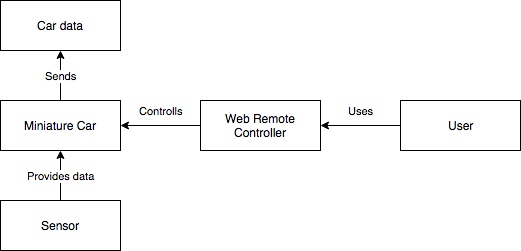
\includegraphics[width=\linewidth]{Diagrams/DomainModel.png}
\caption{Domain Model}
\label{fig:domainmodel}
\end{figure}
\FloatBarrier % -> Wrap image with this, to make sure text does not go infront of image if theres room

%%%%%%%%%%%%%%%%%%%%%%%%%%%%%%
%%% New Subsection    
\subsection{System Interface}
The software provides the user two way of interfacing withthe car; the so called terminal remote controller and the web remote controller. 

The terminal remote controller provides the user with the ability to control the car through a simple computer terminal. Here, the user controls the car through the use of the keys. Furthermore, the user may also set the speed and the steering angle car should have when driving. Lastly, in case an obstacle is detected within a set distance, the car will break.

The more extensive web remote controller provides aforementioned features, (apart from being able to set the steering angle and distance before breaking for obstacles) together with another set of functionalities. Through the web remote controller, the car's speed, heading, distance traveled and the distance to obstacles are presented. In addition, most data that the car sends, receives and processes are displayed in the interface. Lastly, the interface provides the user with a switch that chooses which mode the car shall be in; leader (the user controls the car) or follower (the car follows another car autonomously).

%%%%%%%%%%%%%%%%%%%%%%%%%%%%%%
%%% New Subsection    
\subsection{External Libraries/Images}
To realize our software, various libraries and Docker images were used.

\begin{longtable}{ | p{0.15\linewidth} | p{0.11\linewidth} | p{0.74\linewidth} | }\hline 
	\textbf{Name} & \textbf{Link} & \textbf{Description} \\ \hline
	libcluon & goo.gl/ jwGbj8 & Christian Berger's C++ library libcluon is the hub of our software. It is used for all communication, both internally in the car and externally to other car's.\\ \hline
    seresearch/ 2018-dit-168 & goo.gl/ qR4uqi & From this image we run two microservices, odsupercomponent and the proxy-miniature-pwm-motor which allow our software to control the miniature car through sending messages with the libcluon library.\\ \hline
	opendlv-device-ultrasonic-srf08-armhf & goo.gl/ N4LpsK & This image gets the front ultrasonic sensor's reading and make it available for our code to use.\\ \hline
    Robotics Cape & goo.gl/ D4mynE & This library allows our software to access data readings from the sensors that are placed on the BeagleBone.\\ \hline
\end{longtable}

\pagebreak


%%%%%%%%%%%%%%%%%%%%%%%%%%%%%%%%%%%%%%%%%%%%%%%%%%%
% Adding section detailing architecture motivations
%%%%%%%%%%%%%%%%%%%%%%%%%%%%%%%%%%%%%%%%%%%%%%%%%%%
\section{Architectural Drivers}
\subsection{Functional Requirements}
Functional requirements were used to identify and narrow down the project scope. The requirements are prioritized using MoSCoW notation i.e. requirements are divided into Must, Shoulds, Coulds, and Wont’s. Must dictates requirements that are mandatory for the final demonstration. Should expresses requirements that are significant, but do not have a defined deadline. Could expresses requirements/features that would improve the project quality, but are not necessarily implemented. Lastly, Won’t is used to track identified requirements that will not be implemented, due to product owner dislike or disapproval, time and budgetary constraints.\par

% Functional requirement table
% Define 4 aligned columns; l = left, c = center, r = right, the | = means vertical line    % \hline -> Draw horizontal line
\begin{longtable}{| p{0.05\linewidth} | p{0.15\linewidth} | p{0.45\linewidth} | p{0.25\linewidth} | p{0.1\linewidth} |}\hline 
    ID & Requirement & Description & Status & Priority \\ \hline
   	F1 & Message Log & A web page must contain a message log of everything that has been sent internally and externally within the car & Not Implemented & Must\\ \hline
   	F2 & Remote Controller & A web page must contain a graphical remote controller that communicates and controls Dash, when the car is the leader of the platoon & Not Implemented & Must\\ \hline
   	F3 & Ultrasonics & Dash will support ultrasonic sensors; will be able to broadcast distance sensor data to the local OD4 session & Not Implemented & Must\\ \hline
   	F4 & Leader Connection & The car, Dash, must be able to support Leader functionality (i.e. send LeaderStatus requests) while platooning & Not Implemented & Must\\ \hline       
    F5 & Follower Connection & The car, Dash, must be able to participate in platooning as a follower & Not Implemented & Must\\ \hline
    F6 & Maneuvering & The car will drive forward, turn left or right on commands received over the OD4 session & Not Implemented & Must\\ \hline
   	F7 & IMU & Dash must be able to use the IMU on its BeagleBoard Blue to calculate the distance moved and be able to send that using the V2V Protocol & Not Implemented & Must\\ \hline
   	F8 & V2V Protocol & The car must be able to support the V2V Protocol. It is required for it to communicate with other cars and send sensors data & Not Implemented & Must\\ \hline
   	F9 & Collision Prevention & Dash will stop/brake when ultrasonic readings return an object that is less or equals to 10 cm ahead & Not Implemented & Should\\ \hline
   	F10 & Emergency Brake & The car will stop if it fails to receive 3 update requests (i.e. hasn’t received anything in 300ms) and/or the connection to other cars has been lost & Not Implemented & Must\\ \hline
   	F11 & Video Streaming& The car could incorporate the RPi and camera to live stream it’s video & Not Implemented & Could\\ \hline
  	F12 & Lane Following & Via incorporation of the RPi camera, Dash could implement identification and following of straight lines & Not Implemented & Could\\ \hline
\end{longtable}

%%%%%%%%%%%%%%%%%%%%%%%%%%%%%%%%%%%%%%%%
% Adding section about project use cases
%%%%%%%%%%%%%%%%%%%%%%%%%%%%%%%%%%%%%%%%
\section{Use Case View}
This document section attempts to identify the main behaviour exhibited by Dash. This is done by expressing the behaviour as use case scenarios. The chosen scenarios depicts some of the significant features of developed project. Moreover, the identified scenarios all utilize the V2V Protocol in different aspects, meaning the use case scenarios use different messages from the protocol. Therefore, the identified scenarios fulfil different aspects of the functional requirements of F8 (V2V Protocol). \par

\subsection{Use Case Scenarios}

%%%%%%%%%%%%%%%%%%%%%%%%%%%%%%
%%% Use Case 1 Table
\subsubsection{Connect As Follower}
\begin{longtable}{| p{0.2\linewidth} | p{0.8\linewidth} |}\hline 
    ID & UC1\\ \hline
    Use Case & Connect as Follower\\ \hline
    Description & Dash connects to another miniature car as a Follower and begins to receiving Leader Status update messages\\ \hline
    Actors & Dash, Another Car\\ \hline
    Preconditions & Excluding Dash there is another miniature car with the V2V protocol that are not already connected to any cars\\ \hline
    Steps & Basic Flow: \begin{enumerate} % enumerate creates a numbered list
    	\itemsep 0em % -> Specify gaps between numbers in list 
    	\item Dash uses Announce Presence (it’s not very effective). Another car receives Dash’s IP and group number
		\item Another Car announces presence. Dash receives it’s IP and group number
        \item Dash uses Follow Requests. Selects which group car to follow
        \item Another Car receives follow request and does not have a follower yet. Another Car sends Follow Response
        \item A connection using UDP Sender and Receiver is established between Dash and Another Car 
        \end{enumerate}
        Alternative Flow: \begin{enumerate}
        	\setcounter{enumi}{3} % -> Starts list from a different specified index + 1
        	\item Another Car already has a Follower. 
            \begin{enumerate} % -> nested enumerates, index list. Default index 1->a->i->A
            	\itemsep 0em % -> Specify gaps between numbers in list 
         		\item No Follower Request is sent
         		\item Display a message informing the users
               	\item Continues at Basic Flow 2
       		\end{enumerate}
       	\end{enumerate}\\ \hline
\end{longtable}

%%%%%%%%%%%%%%%%%%%%%%%%%%%%%%
%%% Use Case 2 Table
\subsubsection{Connect As Leader}
\begin{longtable}{| p{0.2\linewidth} | p{0.8\linewidth} |}\hline 
    ID & UC2\\ \hline
    Use Case & Connect as Leader\\ \hline
    Description & Dash connects to another miniature car as a Leader and begins to sending Leader Status update messages\\ \hline
    Actors & Dash, Another Car\\ \hline
    Preconditions & Excluding Dash there is another miniature car with the V2V protocol that are not already connected to any cars\\ \hline
    Steps & Basic Flow: \begin{enumerate} % enumerate creates a numbered list
        \itemsep 0em % -> Specify gaps between numbers in list 
    	\item Dash uses Announce Presence (it’s not very effective). Another car receives Dash’s IP and group number
		\item Another Car announces presence. Dash receives it’s IP and group number
        \item Dash receives follow request and does not have a follower yet. Dash sends Follow Response
        \item Another Car receives follow request and does not have a follower yet. Another Car sends Follow Response
        \item A connection using UDP Sender and Receiver is established between Dash and Another Car 
        \end{enumerate}
        Alternative Flow: \begin{enumerate}
        	\setcounter{enumi}{3} % -> Starts list from a different specified index + 1
        	\item Dash already has a Follower. 
            \begin{enumerate} % -> nested enumerates, index list. Default index 1->a->i->A
            	\itemsep 0em % -> Specify gaps between numbers in list 
         		\item No Follower Request is sent
         		\item Display a message informing the users
               	\item Continues at Basic Flow 2
       		\end{enumerate}
       	\end{enumerate}\\ \hline
\end{longtable}

%%%%%%%%%%%%%%%%%%%%%%%%%%%%%%
%%% Use Case 3 Table
\subsubsection{Stop Following Leader}
\begin{longtable}{| p{0.2\linewidth} | p{0.8\linewidth} |}\hline 
    ID & UC3\\ \hline
    Use Case & Connect as Leader\\ \hline
    Description & Dash disconnect from Another Car, which acted as a Leader\\ \hline
    Actors & Dash, Another Car\\ \hline
    Preconditions & Dash is already connected as a Follower to Another Car\\ \hline
    Steps & Basic Flow: \begin{enumerate} % enumerate creates a numbered list
        \itemsep 0em % -> Specify gaps between numbers in list 
    	\item Dash sends Follower Status and receives Leader Status, indicating it’s following Another Car
		\item Dash sends Stop Following message and stops moving
        \item Dash removes Another Car as it’s leader
        \item Another Car receives stop following message. Another Car removes Dash as it’s follower
	\end{enumerate}\\ \hline
\end{longtable}

%%%%%%%%%%%%%%%%%%%%%%%%%%%%%%
%%% Use Case 4 Table
\subsubsection{Drive Dash}
\begin{longtable}{| p{0.2\linewidth} | p{0.8\linewidth} |}\hline 
    ID & UC4\\ \hline
    Use Case & Drive Dash\\ \hline
    Description & Another Car connects to Dash as a Follower, at which point a Driver uses the remote controller to maneuver Dash\\ \hline
    Actors & Dash, Driver, Another Car\\ \hline
    Preconditions & Another Car is already connected to Dash as a Follower\\ \hline
    Steps & Basic Flow: \begin{enumerate} % enumerate creates a numbered list
        \itemsep 0em % -> Specify gaps between numbers in list 
    	\item ???
	\end{enumerate}\\ \hline
\end{longtable}

%%%%%%%%%%%%%%%%%%%%%%%%%%%%%%
%%% New Subcetion
\subsection{Use Case Diagram}
To depict use case interactions amongst each other, a use case diagram was created. Moreover, the diagram also servers as a visual aid, aimed to improve understanding of actor interactions with project functionality. The diagram depicts the interactions between the most significant use cases, mentioned in previous sections.\par

\FloatBarrier % -> Wrap image with this, to make sure text does not go infront of image if theres room
% Adding use case diagram image
\begin{figure}[ht!]
\centering
% Make image as wide as the line
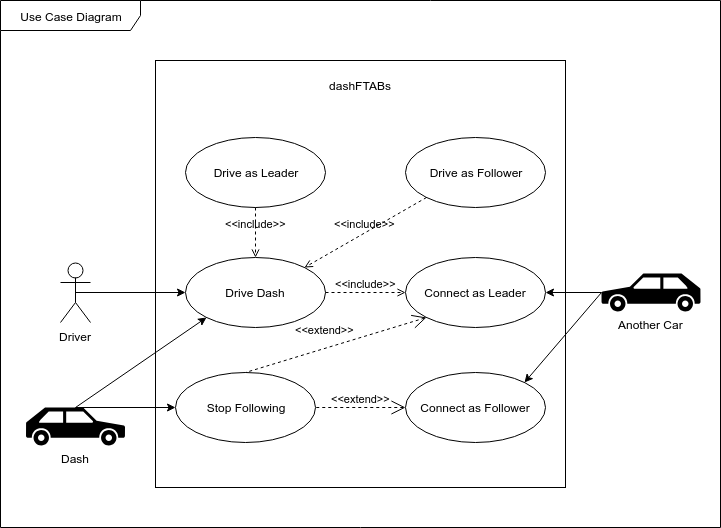
\includegraphics[width=\linewidth]{Diagrams/UseCaseDiagram.png}
\caption{Use Case Diagram}
\label{fig:usecasediagram}
\end{figure}
\FloatBarrier % -> Wrap image with this, to make sure text does not go infront of image if theres room

%%%%%%%%%%%%%%%%%%%%%%%%%%%%%%%%%%%%%%%%%%%%%%%%%
% Adding section about microservice communication
%%%%%%%%%%%%%%%%%%%%%%%%%%%%%%%%%%%%%%%%%%%%%%%%%
\section{Process View}
The Process View section aims to inform the reader on subjects such as communication between the designed software components and communication between the project's subsystem i.e. the developed microservices. The section graphically express the architecturally significant use cases (See section Use Case View). Sequence Diagrams (SD for short) were used for use case realization, while natural language was used to improve the readers’ understanding of the architectural significance the use cases provide.\par

\subsection{V2V Protocol}
As the focus for the project is vehicle-to-vehicle (V2V) communication, a shared V2V protocol was developed by a representative from each team for the purpose of being utilized in the project. The project group dashFTABs has altered the provided protocol to accommodate their team's needs. The changes introduced do not go against any established agreements as the protocol is licensed under GNU General Public License v3.0, a license allowing modification. Moreover, the protocol was design in a way that would require small alterations to accommodative individual teams architecture. Due to the protocol being used by all project groups the behaviour exhibited by Connect as Leader, Connect as Follower will be similar across all teams.\par
The specific changes to the protocol include; creating an additional OD4 session for internal car communication, broadcasting the messages received from other cars to the internal channel, as well as an additional function responsible for monitoring time Leader/Follower Status request have been received. \par  

%%%%%%%%%%%%%%%%%%%%%%%%%%%%%%
%%% Connect As Follower
\subsection{Connect As Follower}
\subsubsection{Significance}
 The use case was chosen as architecturally significant, as it implements functional requirement F5, Follower Connection. The requirement itself was provided by the DIT168 course representatives, as it is mandatory for every miniature vehicle to posses follower capabilities. Without a follower connection, Dash would not be able to have automated moving or platooning, as it would not receive status updates from the leader. Therefore, F5 requirement acts as a prerequisite to more advanced functionality. Due to these reasons the requirement was deemed as significant and expressed as a sequence diagram. The sequence diagram depicts the behavior of UC1.\par

% Adding image
\FloatBarrier % -> Wrap image with this, to make sure text does not go in front of image if theres room
\begin{figure}[ht!]
\centering
% Make image as wide as the line
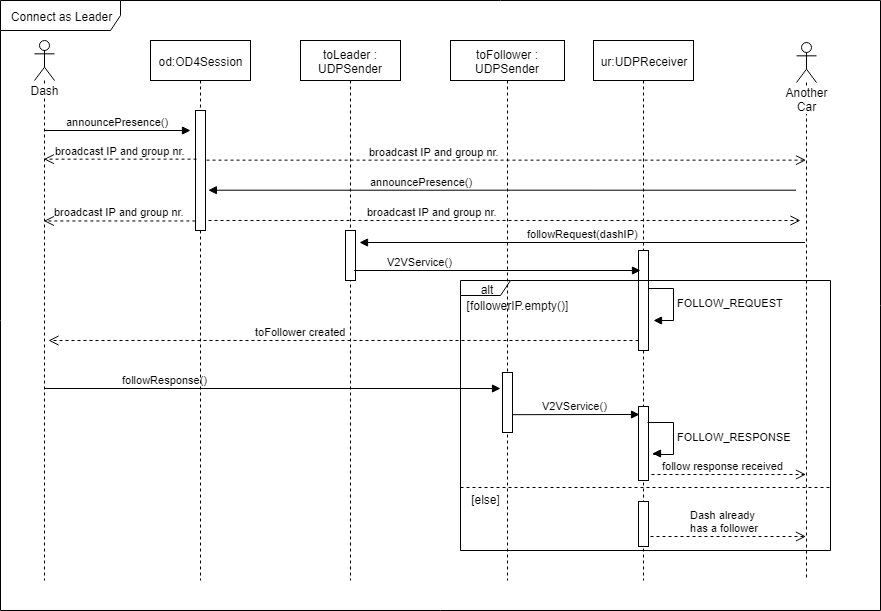
\includegraphics[width=\linewidth]{Diagrams/ConnectAsFollower.png}
\caption{Connect As Follower SD}
\label{fig:connectasfollower}
\end{figure}
\FloatBarrier % -> Wrap image with this, to make sure text does not go infront of image if theres room

\subsubsection{Component Behaviour}
The interactions depicted in Figure \ref{fig:connectasfollower} focus specifically on behaviour exhibited by the V2V microservice. The diagram consists of 5 main components; OD4 Sessions broadcast and internal, UPD Senders toLeader, toFollower, and receiver a UDP Receiver. The broadcast OD4 session listens to CID 250, a channel used for cars that wish to engage in platooning. Once a car has used announcePresence() their car IP and group number are broadcasted to everyone on the network. \par

%%%%%%%%%%%%%%%%%%%%%%%%%%%%%%
%%% Connect As Leader
\subsection{Connect As Leader}
\subsubsection{Significance}
% Adding image
\FloatBarrier % -> Wrap image with this, to make sure text does not go infront of image if theres room
\begin{figure}
\centering
% Make image as wide as the line
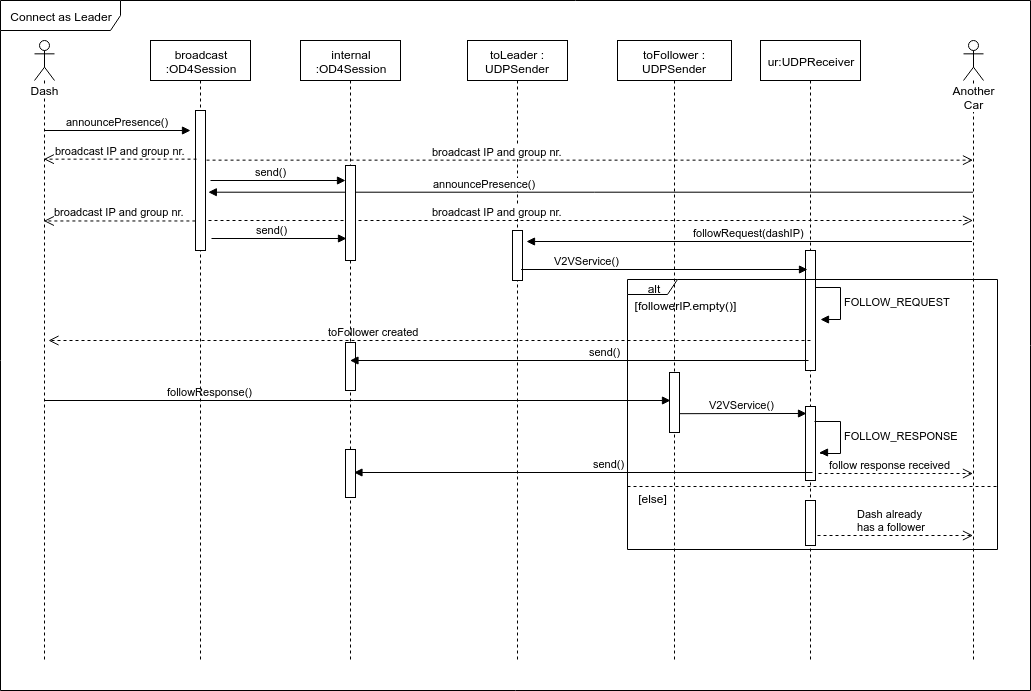
\includegraphics[width=\linewidth]{Diagrams/ConnectAsLeader.png}
\caption{Connect As Leader SD}
\label{fig:stopfollowing}
\end{figure}
\FloatBarrier % -> Wrap image with this, to make sure text does not go infront of image if theres room

%%%%%%%%%%%%%%%%%%%%%%%%%%%%%%
%%% Stop Following
\subsection{Stop Following}

% Adding image
\FloatBarrier % -> Wrap image with this, to make sure text does not go infront of image if theres room
\begin{figure}
\centering
% Make image as wide as the line
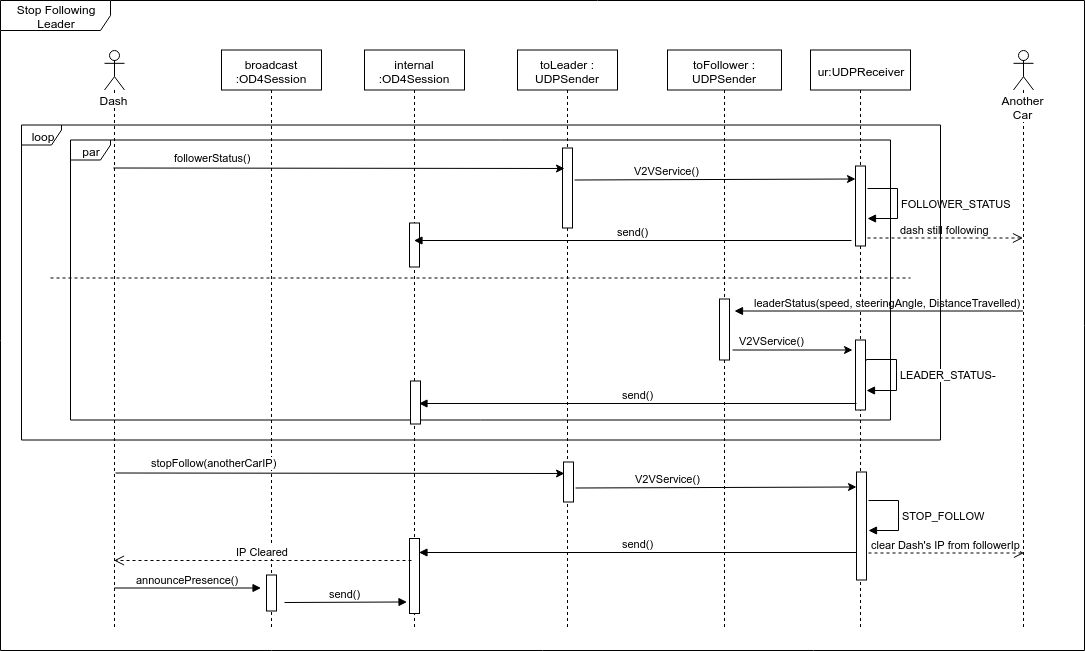
\includegraphics[width=\linewidth]{Diagrams/StopFollowing.png}
\caption{Stop Following SD}
\label{fig:connectasleader}
\end{figure}
\FloatBarrier % -> Wrap image with this, to make sure text does not go infront of image if theres room


\end{document}
